
\chapter{School Financing in California}\label{ch:ca-school-financing}

This appendix presents an example of public school financing in California.\footnote{For a more detailed look at what a complete budget document looks like, see ``LASD 2022–23 Annual Budget'' of Item H.4 of the June 13, 2022 LASD Board Meeting (\url{https://tinyurl.com/lasd-2022--23-annual-budget}). Note that most public school budget documents are not as comprehensive or as well put together as LASD's are.} %chxtex 8
Understanding the normal, usual, default financing of schools in California is necessary in order to be able to identify where Rocketship's might differ. The description which follows is necessarily high-level; the budget document for 2022–23 that LASD submits to SCCOE and hence to the state runs to 118 pages of unadorned tables derived from accounting spreadsheets.

First, the highest possible level look at a LASD budget is presented. This is the \textit{All Funds Summary}. Next are five tables that delve one level down from the \textit{All Funds Summary}. Each of those tables can be further decomposed until individual SACS accounting (object) codes are reached. SACS code reflect exactly one kind of expenditure or revenue. For example, money received from the Federal Emergency Management Agency (FEMA) is recorded under SACS object code 8281 and no where else. How that money is spent is recorded under object code 8285. The lowest level of accounting is money received or money paid. All money received goes into at least one fund and is recorded under at least one object code. Payments are handled correspondingly. The intent of this process is to record unambiguously and completely every monetary transaction. 

Public school districts and charter schools receive funding from the state and the federal governments which most often goes into a district's or school's General Fund. A portion of funding is restricted to particular programs, and sometimes that money goes into a specialized and restricted fund, but the norm is for the General Fund to account for the majority of transactions.

The first table to look at is the aggregate of all funds as shown in \prettyref{fig:LASD_All_Funds_Summary}. It is a very high-level summary of a school's or a district's budget. It's a snapshot of what the district's revenues are expected to be, roughly where that revenue is expected to come from, what the district's expenses are expected to be, and whether revenue and expenses are expected to be in balance. It is the rough equivalent of a business income statement.\footnote{Schools group their finances by funds. Most of their revenue goes into the general fund, and most of their expenses come out of the general fund. Some transactions must by law be accounted for in different funds. The three largest funds are the General Fund, the Special Revenue Fund, and the Capital Projects Fund, and together they account for virtually all of the financial activity of LASD.\@ Other schools may have a different set of funds, but all contain a General Fund that is the primary fund for their day-to-day financial activities.}

\begin{figure}
  \centering
  \caption[LASD 2019–20 All Funds Summary]{\textit{LASD 2019–20 All Funds Summary}}\label{fig:LASD_All_Funds_Summary}
  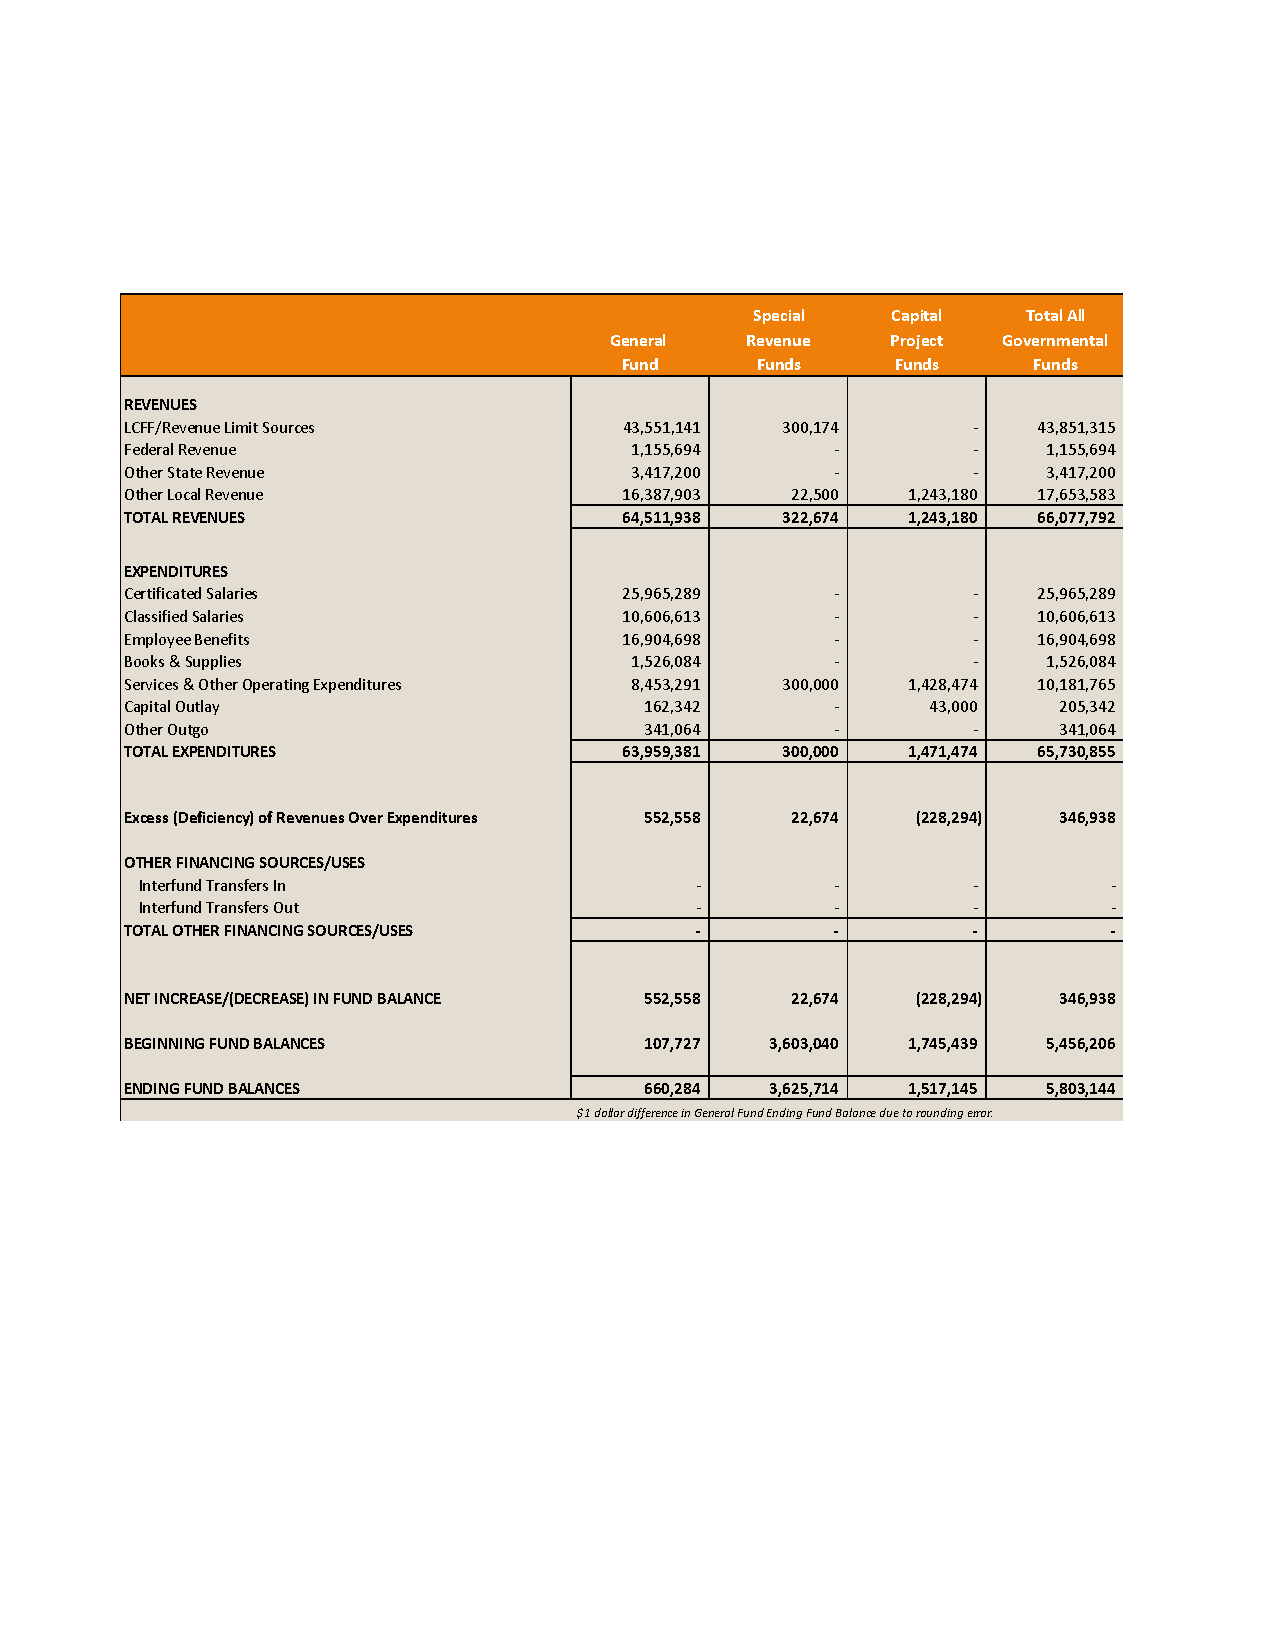
\includegraphics[width=\textwidth]{LASD_2019-20_All_Funds_Summary}\\ %chktex 8
  \footnotesize\raggedright\textcite[38]{Kenyon2019}.
\end{figure}

Because Figure~\ref{fig:LASD_All_Funds_Summary},~\titleref{fig:LASD_All_Funds_Summary}, is a snapshot, detecting unusual changes year-to-year is not possible. Changes are detectable using  \prettyref{fig:net-position} which compares fiscal two years. However, with just a budget summary, one can nonetheless note some interesting ratios, for example, the percentage of expenses spent on salaries and benefits. For LASD in 2021–20, this is 80.18\% which is in line with what is typical of elementary school districts in California. One can calculate the state-wide average for all districts for 2019–20 using the Data Table at \url{www.ed-data.org/state/CA}, and that comes out to 83.71\%. So, LASD spends a little less on salaries and benefits than the average elementary school district in California does.

Calculating this ratio brings up a general issue: What is an appropriate comparison group? In this particular case, the Ed-Data web site does not have county-level financial data, so the only comparison which can easily be made is at the state level. But should the state-level comparison group be all districts, or just elementary school districts? Should ``basic aid'' districts, also called ``community-funded'' districts, districts whose property tax revenues exceed their LCFF entitlement, be included or not? Again, the Data Table tab on \url{www.ed-data.or/state/CA} does not filter by type of district (although the Graph tab does), so, in this case, using just the Ed-Data data, our choices are forced since we cannot use state-level data.

The other common financial business report is the balance sheet, which identifies assets and liabilities. In the educational world, this is the statement of net position. \prettyref{fig:net-position} shows LASD's assets and liabilities at the end of the 2019–20 school year. Note that unlike a balance sheet, a statement of net position for schools (and other governmental entities) does not balance; assets are not exactly equal to liabilities.\footnote{Business accountants achieve this seemingly low probability equality by adding a fudge factor, \textit{owner's equity}, so that \texttt{\textit{assets = liabilities + equity}} always, exactly.}

As an example of a number which stands out and is therefore worth investigating, is the large increase in Capital Assets, year over year, an increase of \$132M (line 3 of \prettyref{fig:net-position}). In \citetitle{Kenyon2021}, six notes appear immediately after Figure~\ref{fig:net-position}, and these provide an explanation for the increase: LASD purchased a property whose cost was \$134.9M net of \$2.7M in depreciation. This purchase shows up again in line 1 of \prettyref{fig:Capital_Assets} and explains the enormous 9052\% increase in the value of LASD's largest asset in FY2019, land.

In addition, the \citetitle{Kenyon2021} contains a section, on pp. 19–45, called \textit{Notes to the Basic Financial Statements}. Theses notes are an integral part of the certified, audited annual statement, just as they are in audited financial reports in the business world; they cannot be omitted, and must be accurate and complete.  Note 7B of \textcite[7]{Kenyon2021}, General Obligation (GO) Bond Anticipation Notes (BANs), explains how LASD uses a common
technique to convert general obligation bonds into cash: issue BANs, backed by general obligation bonds, and payable when those GO bonds are issued.\footnote{One reason this makes sense is that interest rate on BANs is less than the interest rate of GO bonds, so LASD makes money by issuing BANs to pay off GO bonds. In a different situation, school districts issue tax revenue anticipation notes (TRANs) because property taxes are paid by taxpayers semi-annually and salaries are paid monthly, so districts often and predictably do not have the cash on hand to pay their employees. The solution is to issue TRANs backed by anticipated revenue, and are paid off when the school or district receives the funds.}

It's important to remember is that although changes in finances can be complicated, they should also be adequately explained in a transparent and complete CAFR\@. When the documents are incomplete or opaque is when serious concerns should be raised. % chktex 13

Within a CAFR are five summaries of financial tables that go one level deeper than the All Funds Summary. These are
\begin{itemize}\OnehalfSpacing%
    \item Summary of Net Position (\prettyref{fig:net-position})
    \item Change in Net Position  (\prettyref{fig:Change_Position})
    \item Net Costs of Services   (\prettyref{fig:Cost_Services})
    \item Capital Assets          (\prettyref{fig:Capital_Assets})
    \item Long-term Liabilities   (\prettyref{fig:Long-term_Liabilities})
  \end{itemize}

\begin{figure}
  \centering
  \caption[LASD YE 2020 Summary of Net Position]{\textit{LASD YE 2020 Summary of Net Position}}\label{fig:net-position}
  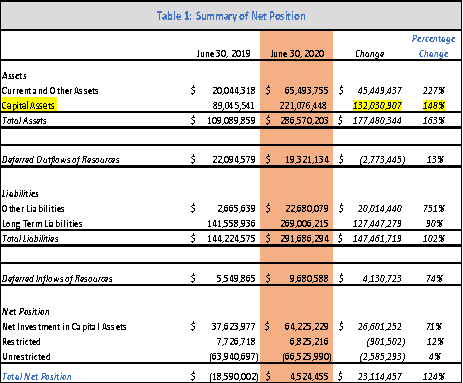
\includegraphics[width=\textwidth]{CAFR-YE2020_Summary_of_Net_Position}\\
  \footnotesize\raggedright\textcite[6]{Kenyon2021}.
\end{figure}

\begin{figure}
  \centering
  \caption[LASD YE 2020 Change of Net Position]{\textit{LASD YE 2020 Change of Net Position}}\label{fig:Change_Position}
  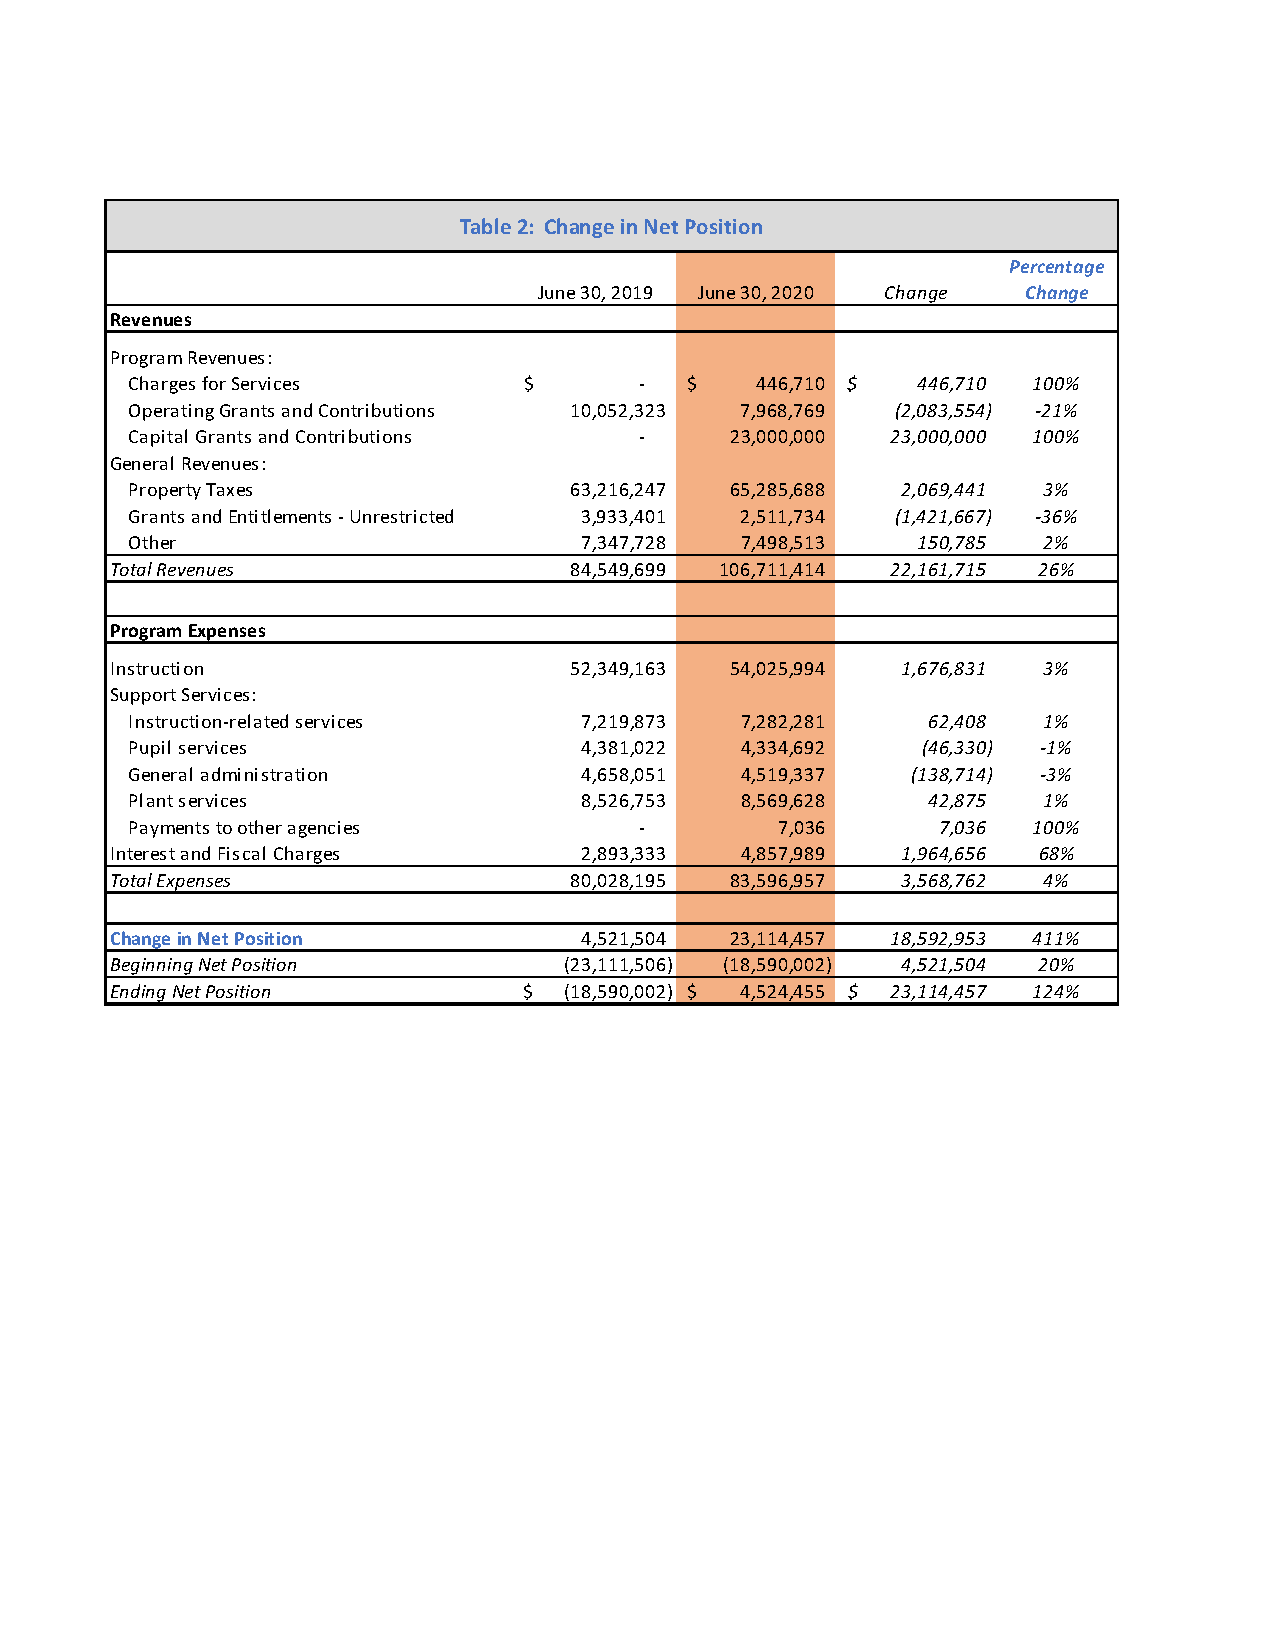
\includegraphics[width=\textwidth]{CAFR-YE2020_Change_in_Net_Position}\\
  \footnotesize\raggedright\textcite[7]{Kenyon2021}.
\end{figure}

\begin{figure}
  \centering
  \caption[LASD YE 2020 Net Cost of Services]{\textit{LASD YE 2020 Net Cost of Services}}\label{fig:Cost_Services}
  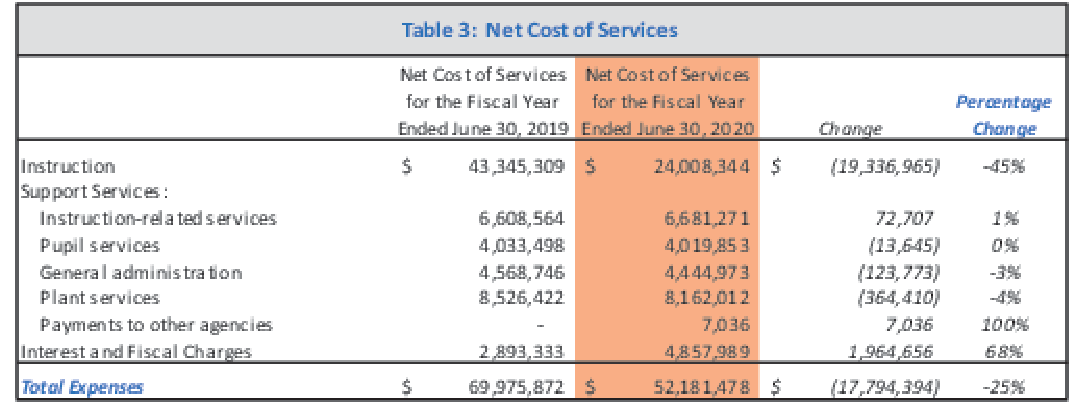
\includegraphics[width=\textwidth]{CAFR-YE2020_Net_Cost_of_Services}\\
  \footnotesize\raggedright\textcite[9]{Kenyon2021}.
\end{figure}

\begin{figure}
  \centering
  \caption[LASD YE 2020 Capital Assets]{\textit{LASD YE 2020 Capital Assets}}\label{fig:Capital_Assets}
  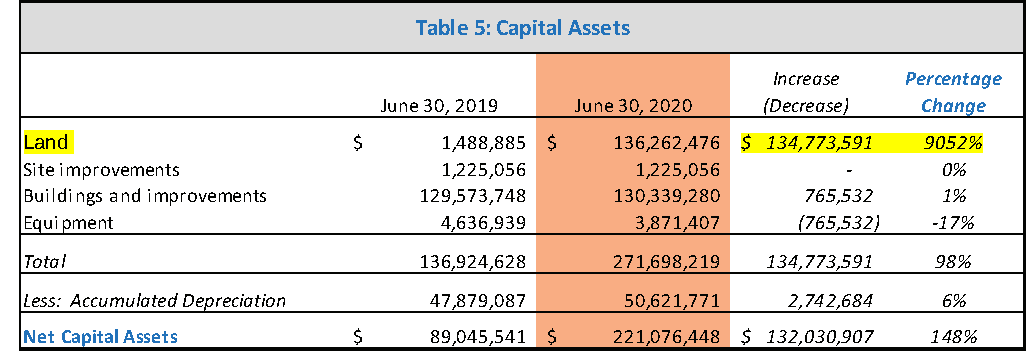
\includegraphics[width=\textwidth]{CAFR-YE2020_Capital_Assets}\\
  \footnotesize\raggedright\textcite[10]{Kenyon2021}.
\end{figure}

\begin{figure}
  \centering
  \caption[LASD YE 2020 Long-term Liabilities]{\textit{LASD YE 2020 Long-term Liabilities}}\label{fig:Long-term_Liabilities}
  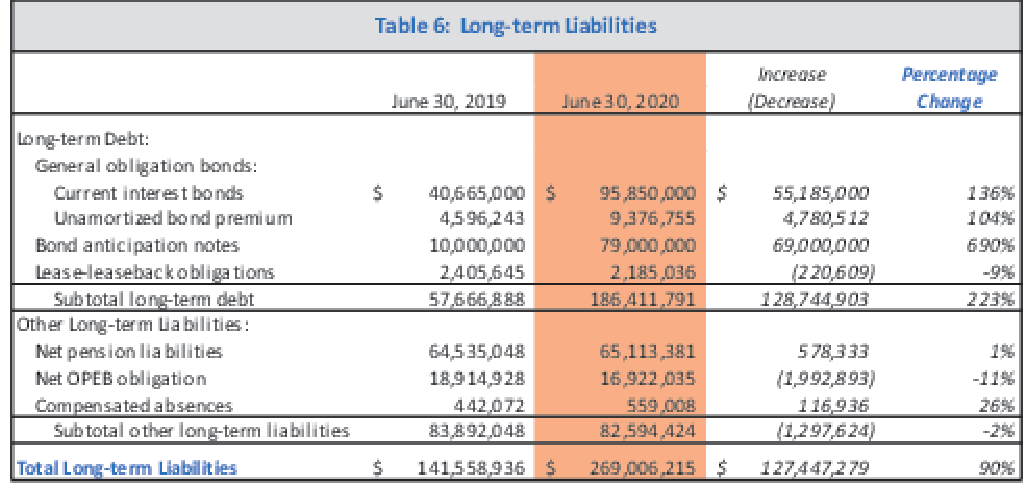
\includegraphics[width=\textwidth]{CAFR-YE2020_Long-term_Liabilities}\\
  \footnotesize\raggedright\textcite[11]{Kenyon2021}.
\end{figure}%

LASD rolls up its detailed financial data into a single multi-year summary, as shown in \prettyref{fig:multi-year-proj}. In addition to purely financial data, the multi-year summary includes the key
assumptions that were behind the numbers. In fact, the first section of Figure~\ref{fig:multi-year-proj} is only assumptions, and it is those assumptions which drive the numbers in Sections 2–4. The value of this summary is that it captures in one table the key data needed to make budgetary decisions and thus might serve as a template for what data is important. 

\begin{figure}[!t]
  \centering
  \caption[LASD 2019–20 Multi-Year Projection]{\textit{LASD 2019–20 Multi-Year Projection}}\label{fig:multi-year-proj}
  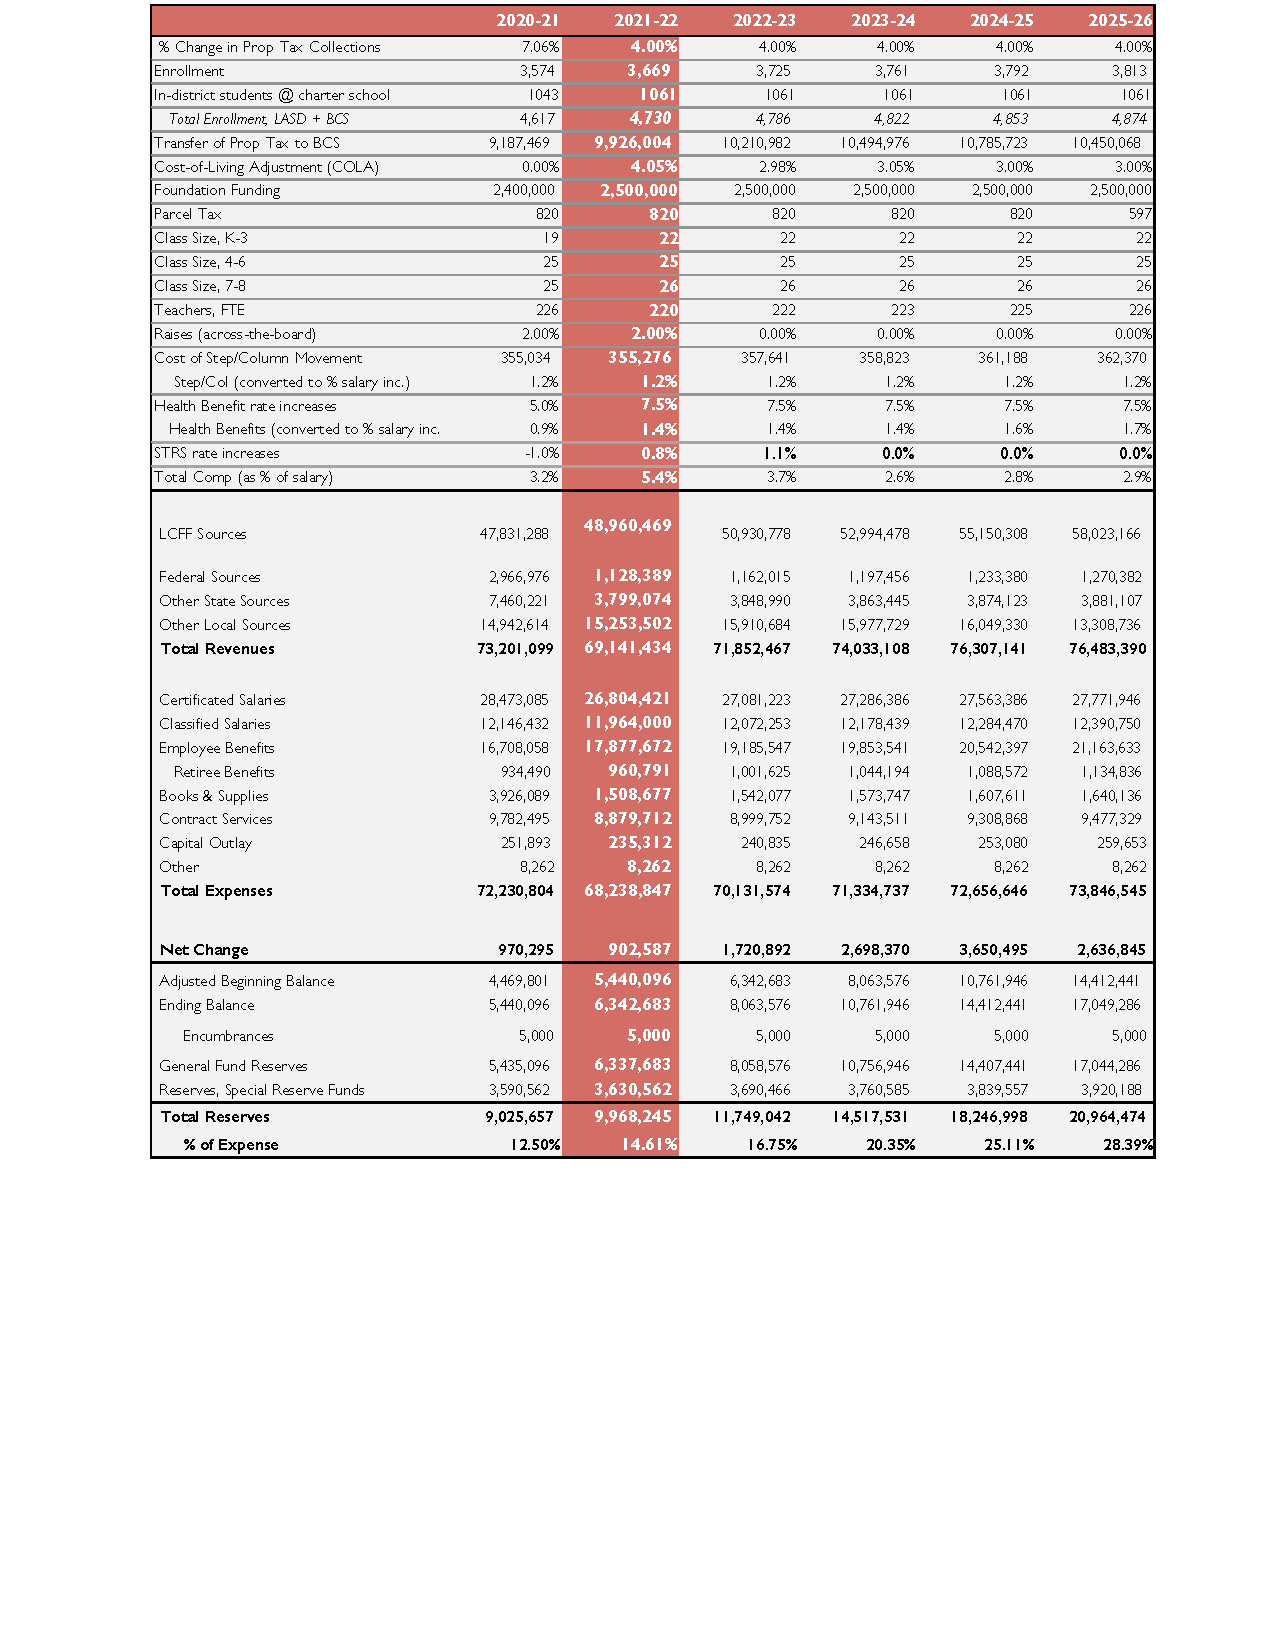
\includegraphics[width=\textwidth]{LASD_Multi_Year_Projection}\
  \footnotesize\raggedright\textcite[137]{Kenyon2021a}.
\end{figure}\bigskip%


%%% Local Variables:
%%% mode: latex
%%% TeX-master: "Rocketship_Education-An_Exploratory_Public_Policy_Case_Study"
%%% End:
